\setcounter{chapter}{0}
\setcounter{section}{0}
\chapter{Introduction}
\setlength{\headheight}{12.71342pt}
\addtolength{\topmargin}{-0.71342pt}

\section{Problem Description}
Protein is one of the macronutrients which primarily makes up tissue building in the human body. Furthermore, the macronutrient is indispensable in many other physiological functions, such as hormones, immune system, and other regulatory mechanisms (Ferrari et al., 2022). The recommended daily allowance of protein varies between 0.8 - 1.6 g/kg body weight, depending on factors such as physical activity, age, gender etc. (Philips et al., 2016).

\vspace{1em}
With an increasing population and an estimate of almost 10 billion by 2050. The future protein demand is projected to increase as a correlated factor to the population increase (Henchion et al., 2016). Proportionally, Makkar et al. 2014 predicts an increase in animal consumption of 60-70\%. The increasing demand for animal protein risks further extending planetary boundaries and resulting in conflicts related to sustainability. The planetary boundaries framework by the Potsdam Institute for Climate Impact Research defines “a safe operating space for humanity”. It maps out nine Earth system processes critical for maintaining the planet's stability and resilience, processes which are all affected by the Anthropocene (Figure 1) (Richardson et al. 2023).

\begin{figure}[H]
    \centering
    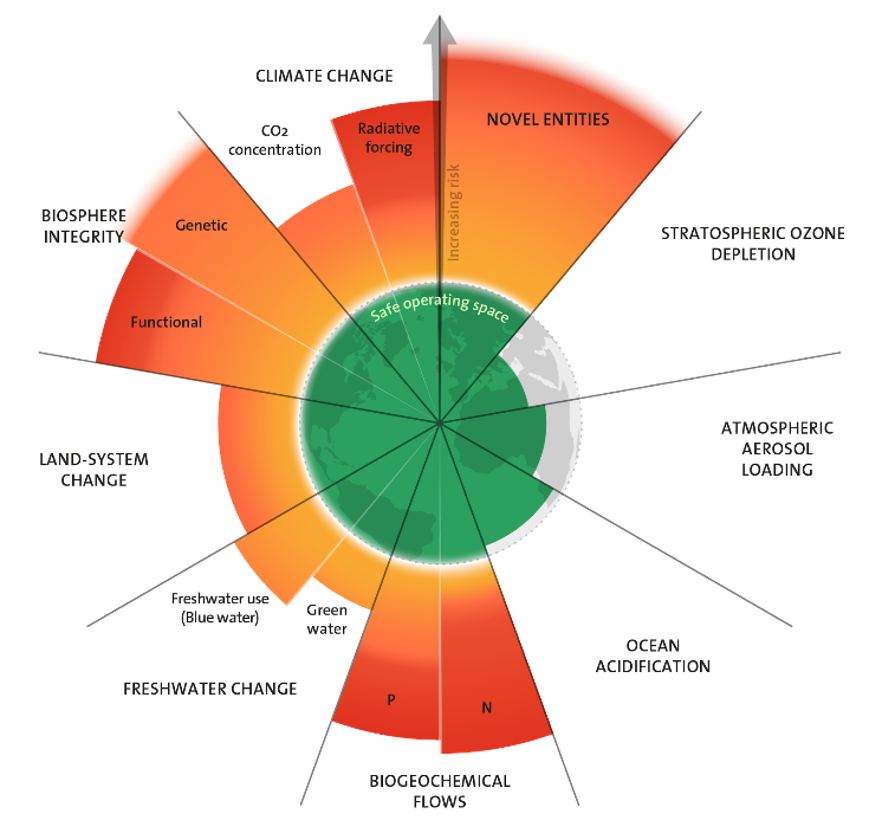
\includegraphics[width=0.58\textwidth]{Figures/fig_01.png}
    \caption{Schematic of the nine Plantary Boundries. (Richardson et al. 2023).}
    \label{fig:introduction_01}
\end{figure}

Thus, humanity stands in front of a challenge in sustaining the supply of animal proteins. Meanwhile, the EAT-Lancet commission declares numerous arguments for a protein shift towards plant-based alternatives. Where human health and environment are two pillar arguments of the diet recommendations (Willett et al., 2019).

\subsection{Aim and Objectives}
The scope of this report narrows down to a nutrient-rich product with low water impact and low CO2  footprint. The formulation targets two of the nine planetary boundaries, freshwater change and CO2-concentration. This report aims to present a hemp protein bar, which served as an alternative to animal-source protein bars, which could help in mitigating the transgression of these planetary boundaries. 

\section{Market Trends \& Target Consumer Group}
With animal sourced protein risking straining the planets' resources, a shift in the traditional diet of the Nordic countries has been studied. On the very subject, Geirsdóttir et al. 2023 provided a thorough scoping-review on Nordic Nutrition Recommendations. They concluded that a shift towards a more plant-based protein diet would benefit both health and the environment. Hence, given the need for a shift, the demand for plant-based protein is expected to increase, while the European meat consumption is expected to decline, the consumption still exceeds that of the respective countries' national recommendations (typically 300-500 g/week). (OECD/FAO, 2023) The Smart Protein Project collects data which helps understanding the status and attitude towards a plant-based diet in various European Countries. Among many surveys, it is stated that “Plant-based sweets, meat alternatives, and milk substitutes emerge as the most sought-after categories for expanding plant-based options.” This accounts for 27\% of the cohorts “express for desire” of such product. Among the top 6 drivers for choosing these products, “health” and “environmentally friendly” are mentioned (45\% and 21\% respectively) (ProVeg, 2023). 

\vspace{1em}
Looking at market predictions and current trends, the global growth of plant-based protein supplements is currently outpacing the growth of that animal source. Which yet again correlates with the future need for sustainable plant-based protein (Market.us, 2024). The consumption of such is seen in either ready-to-eat products or supplements as concentrates or isolates. It is shown that nutritious / functional protein bars are an emerging market as in 2023, it was worth 0,92 billion \$ in Europe. Offering a convenient, ready-to-eat alternative to reach fitness goals. The main consumers of such products are found to be Millennials and Generation Z, with enthusiasm over high protein bars (PW, 2024). Hence, targeting younger consumers is of interest. Furthermore, a plant-based protein bar would target any consumer interested in reducing animal consumption, complementing their daily protein intake, and supplementing regular meals.

\subsection{Existing Market}
As development of plant-based fitness supplements and ready to eat products are increasingly popular, a wide range of products are available. Below is a showcase of an Estonian and Finnish producer, which specialize in hemp-based products and/or raw material. A showcase of a current hemp bar product is also presented.

\subsubsection*{Nordic Hemp, Estonia}
Specializes in organic industrial hemp growing and processing of raw material. Production of 6000 ha / year. (Nordic Hemp, 2025)
\begin{itemize}
    \item Sorting
    \item Dehulling
    \item Processing
    \item Protein isolation
\end{itemize}

\subsubsection*{Impolan Kasvitila, Finland}
Impola plant farm is a family-owned company in its fourth generation. (Impolan Lasvitila, 2025)
They grow and produce product for end-consumers. 

\begin{minipage}{0.6\textwidth}
    \begin{itemize}
        \item Pet and Feed products
        \item Pressing
        \item Dehulling
        \item Hemp chocolate
        \item Hemp muesli
        \item Hemp meal
    \end{itemize}
    \end{minipage}%
    \hfill
    \begin{minipage}{0.35\textwidth}
        \centering
        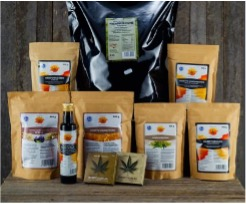
\includegraphics[width=\linewidth]{Figures/fig_02.jpg}
        \captionof{figure}{Hemp protein bar by Nordic Hemp. Selection of products from Impolan Kasvitila, Finland.}
        \label{fig:introduction_02}
    \end{minipage}

\subsubsection*{ROO'bar by Smart Organic, Bulgaria}
Roobar is the flagship brand by Smart Organic AD. They are the largest producer of “minimalistic plant-based bars.” They focus on “... 4-5 ingredients… organic, vegan, raw, and gluten-free”. The production is estimated to 1 million bars per month, and they are accessible in around 50 countries. (Smart Organic, 2025)
\begin{wrapfigure}{r}{0.3\textwidth} 
    \centering
    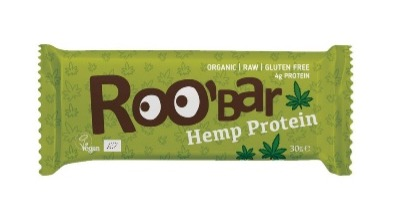
\includegraphics[width=\linewidth]{Figures/fig_03.jpg}
    \caption{ROO'bar Hemp protein bar}
    \caption*{Roobar Hemp protein bar}
    \label{fig:introduction_03}
\end{wrapfigure}


\begin{itemize}
    \item Broad range of different bar products
    \item Owner of a wide range of ready to eat brands
\end{itemize}


\begin{wraptable}{l}{0.5\textwidth} 
    \centering
    \caption{Ingredients: Dates, almonds, hemp protein (18\%). Nutrient declaration per 100 g.}
    \label{tab:your_label}
    \begin{tabular}{|l|l|} 
        \hline
        Energy & 1582 kJ/377kcal \\ 
        \hline
        Fat & 11 g \\ 
        \hline
        - Fatty acids & 1.9 g \\ 
        \hline
        Carbohydrates & 49 g \\ 
        \hline
        - Sugars & 33 g \\ 
        \hline
        - Dietary Fibers & 11 g \\ 
        \hline
        Protein & 14 g \\ 
        \hline
        Salt & 0 g \\ 
        \hline
    \end{tabular}
\end{wraptable}

